\section{Experimental Evaluations}\label{sec:Experiments}

We deploy an HDFS cluster to evaluate EarnCache's performance, on which Spark and EarnCache are deployed as the upper-level application tier and the middle-level caching tier respectively.
The cluster consists of five Amazon EC2 m4.2xlarge nodes, one of which serves as master and the other four serve as slaves.
Each cluster node has 32GB of memory, 12GB reserved as working memory and the remaining 20GB of memory employed as cache resources, summing up to 80GB of cache in total.

We mainly evaluate EarnCache's performance by issuing jobs from Spark to scan files parallelly without any further processing, and compare the performance of EarnCache, the incremental caching, with on-demand style LRU and LFU, and MAX-MIN fair caching.
We set the observation window size of EarnCache to 1000GB by default. For each experiment, we issue file scanning jobs against three files, denoted as FILE-1, FILE-2 and FILE-3, with the following three various frequency patterns, denoted as ROUND, ONE and TWO respectively.
\begin{itemize}
\item ROUND Three files are accessed in pattern: FILE-1, FILE-2,FILE-3 ..., where three files are accessed with equal frequency.
\item ONE Three files are accessed in pattern: FILE-1, FILE-2, FILE-1, FILE-3 ..., where one file is accessed more frequently than other two files.
\item TWO Three files are accessed in pattern: FILE-1, FILE-2, FILE-1, FILE-2, FILE-3 ..., where two files are accessed more frequently than the other file.
\end{itemize}

We set the size of FILE-1, FILE-2 and FILE-3 equally to 40GB and unequally to 70GB, 40GB and 10GB respectively, and then evaluate EarnCache with different caching strategies and frequency patterns. Fig.~\ref{fig:2-a} and Fig.~\ref{fig:2-b} shows the averaged overall running time of jobs. Each column involves scanning equal- or unequal- sized files within one period of the ROUND, ONE or TWO frequency pattern, each including processing of $3$, $4$, and $5$ files. 
We can see that EarnCache produces the best file scanning performance, which exceeds that of the LRU and LFU on-demand caching by a large margin, and leads the MAX-MIN fair caching by a smaller margin. 
The reason of EarnCache achieving the best performance is straight-forward, as most blocks are accessed from memory.
Meanwhile we also observe that the performance of EarnCache is not as mighty as we have expected, especially compared with LRU and LFU on-demand caching.
The reasons are twofold: ~1) EarnCache could not hold all blocks in cache, and file scanning jobs are speeded up partially as a result; ~2) cache-locality is not guaranteed, and a prohibitive number of blocks are accessed from remote cache, rather than local cache.

\begin{figure}[!htbp]
    \subfigure[Files with equal size]{
    		\begin{minipage}[b]{0.43\linewidth}
    		\centering
    		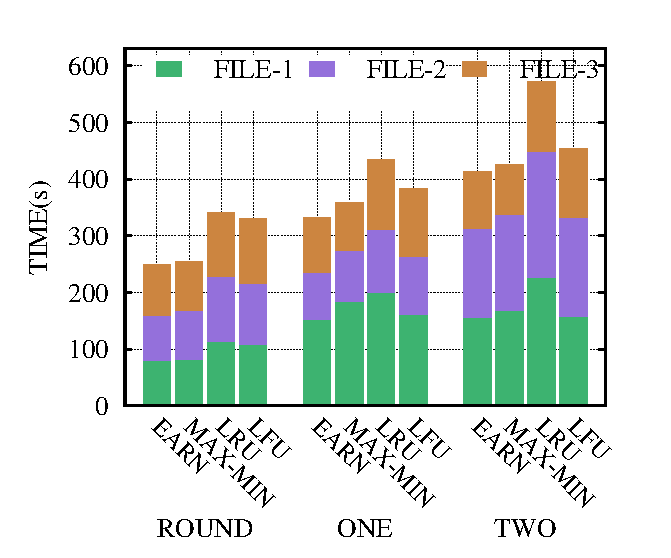
\includegraphics[scale=0.35]{figures/scan444_time_all.eps}
            \label{fig:2-a}
    		\end{minipage}
    }
    \subfigure[Files with unequal size]{
        \begin{minipage}[b]{0.43\linewidth}
        \centering
        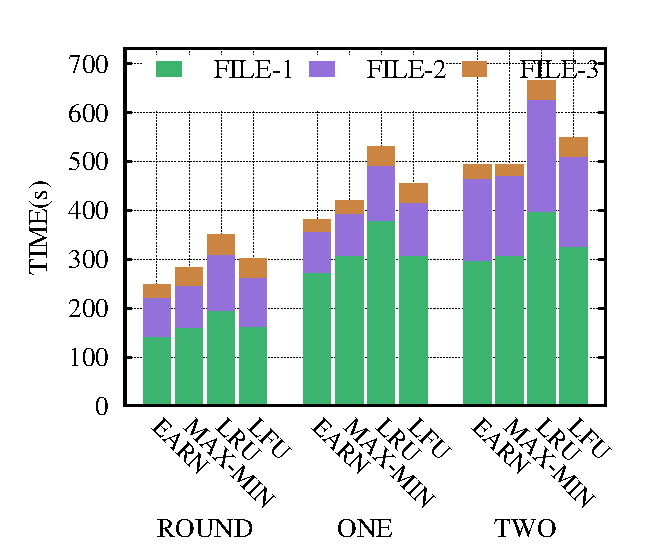
\includegraphics[scale=0.35]{figures/scan741_time_all.eps}
        \label{fig:2-b}
        \end{minipage}
    }
    \caption{Running time of file scanning jobs.}
    \label{fig:2}
\end{figure}

We analyze the distribution of blocks accessed from local cache, remote cache, and the under file system respectively in detail, and the results are shown in Fig.~\ref{fig:block_count}. We can see that EarnCache has the largest number of blocks accessed from cache, whether locally or remotely, which means that it yields the highest memory efficiency than other caching strategies, and this self-evidently explains why EarnCache yields the best file scanning performance. However, we observe that EarnCache has the largest number of blocks accessed from remote cache among the four evaluated strategies. This means EarnCache has the largest potential of performance improvement. If cache-aware task scheduling can be integrated into the upper-level task scheduler, more blocks will be accessed from local cache and EarnCache could obtain much better overall performance then.

\begin{figure}[!htbp]
    \centering
    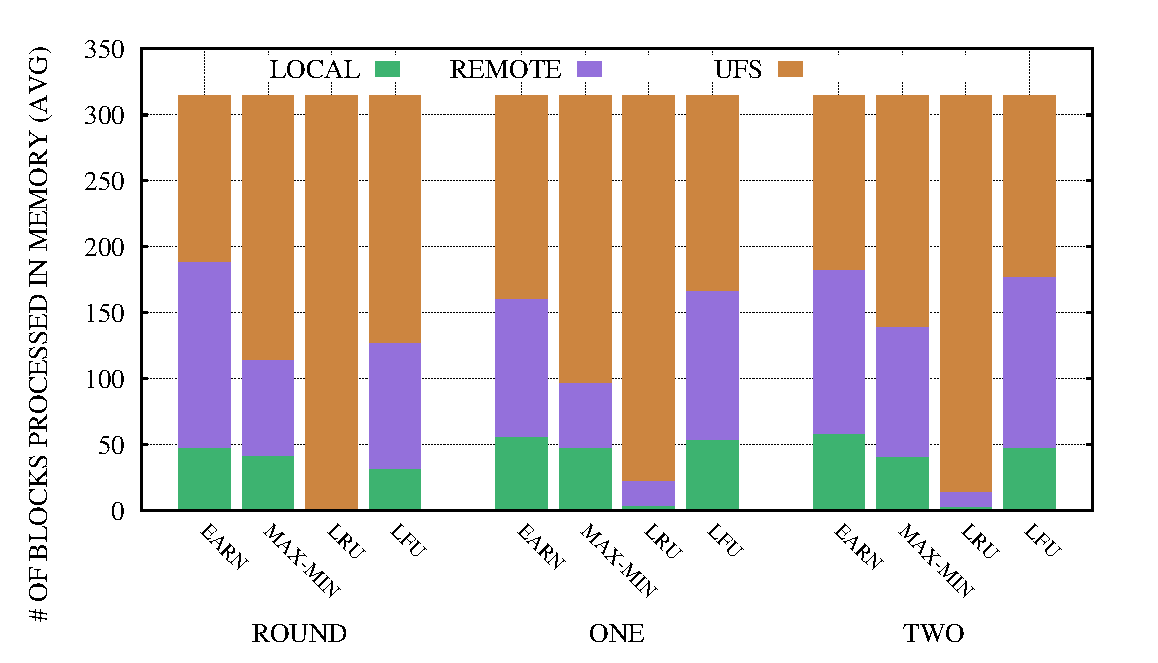
\includegraphics[scale=0.4]{figures/block_count_avg.eps}
    \caption{Distribution of blocks accessed in local cache, remote cache and under file system.}
    \label{fig:block_count}
\end{figure}

Another observation is that the performance of EarnCache is only slightly better than the MAX-MIN caching strategy, and sometimes they achieve similar performance. This is because file receives moderately divergent amounts of cache resources with these two caching strategies, as far as our experimental settings are concerned. 
However, the MAX-MIN caching is unable to dynamically re-allocate resources properly when there exist files not receiving any further accesses. 
To illustrate this, we present the process of resource re-allocation of EarnCache and the MAX-MIN caching in Fig.~\ref{fig:3-2-a} and Fig.~\ref{fig:3-2-b}, where two out of three equal-sized files stop receiving further accesses. We can see that the file remaining accessed gradually takes over cache resources from those obsolete files with time going, while with MAX-MIN fair caching, files still holds almost equal amount cache resources.
Correspondingly, the running time of each job gradually decreases with EarnCache, yet remains stable with MAX-MIN strategy.

%\begin{figure}[!htbp]
%    \subfigure[EARN]{
%    		\begin{minipage}[b]{0.47\linewidth}
%    		\centering
%    		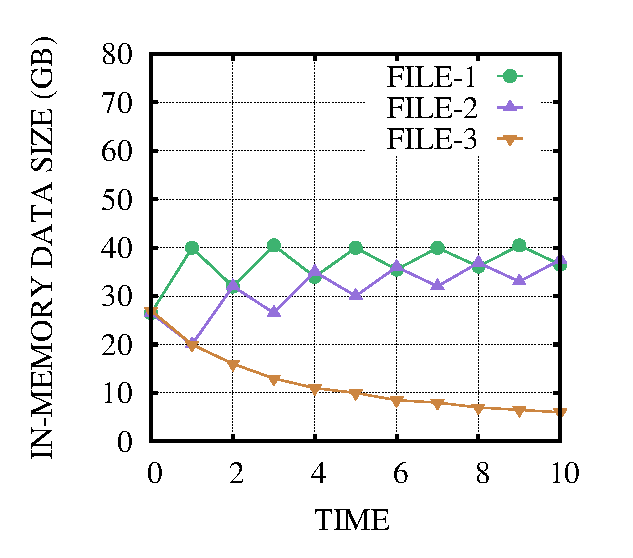
\includegraphics[scale=0.41]{figures/3-1-earn-1000-ds.eps}
%    		\end{minipage}
%    }
%    \subfigure[MAX-MIN]{
%        \begin{minipage}[b]{0.47\linewidth}
%        \centering
%        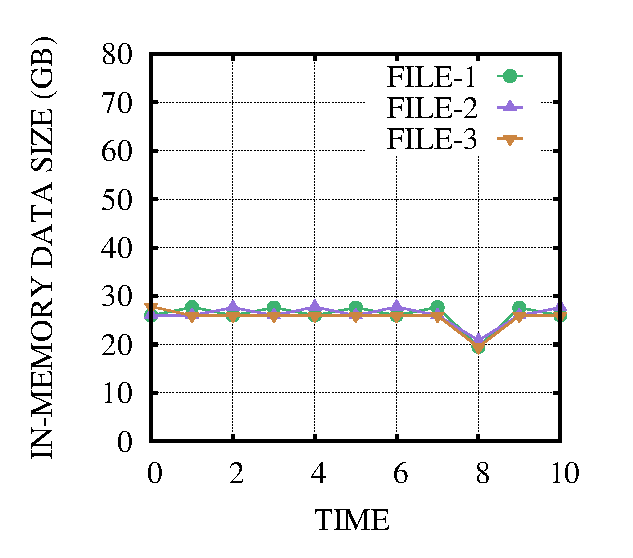
\includegraphics[scale=0.41]{figures/3-1-maxmin-1000-ds.eps}
%        \end{minipage}
%    }
%    \caption{Cache resource In-memory data size of each file after File-3 stops been visited.}
%    \label{fig:3-1}
%\end{figure}


\begin{figure}[!htbp]
    \subfigure[EarnCache]{
    		\begin{minipage}[b]{0.47\linewidth}
    		\centering
    		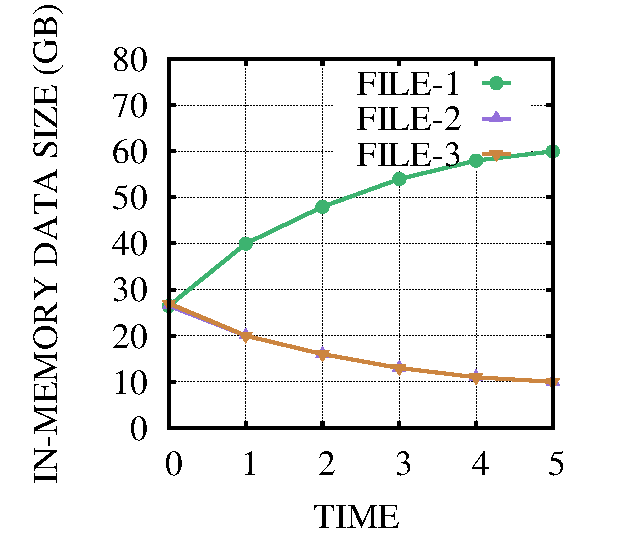
\includegraphics[scale=0.41]{figures/3-2-earn-1000-ds.eps}
            \label{fig:3-2-a}
    		\end{minipage}
    }
    \subfigure[MAX-MIN]{
        \begin{minipage}[b]{0.47\linewidth}
        \centering
        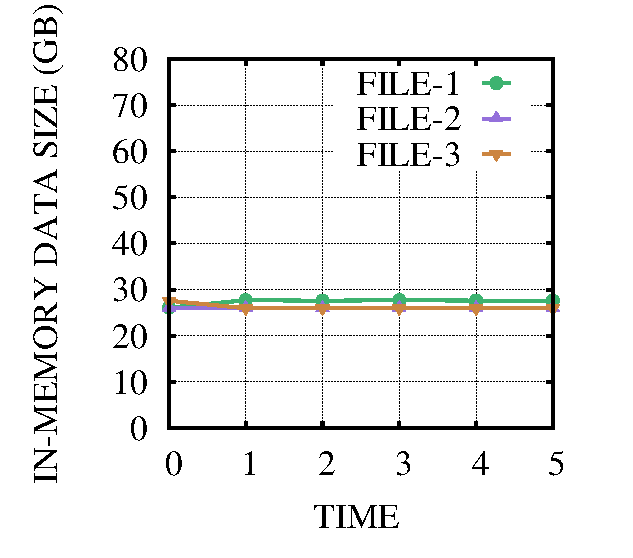
\includegraphics[scale=0.41]{figures/3-2-maxmin-1000-ds.eps}
        \label{fig:3-2-b}
        \end{minipage}
    }
    \caption{Dynamic resource re-allocation with two files receiving no further accesses.}
    \label{fig:3-2}
\end{figure}

Finally, we experimentally analyze the impact of the predefined observation window size on performance, and the results are presented in Fig.~\ref{fig:time_windowsize}.
When observation window is too small, the overall cache efficiency and performance degrades greatly cause competition for cache resources is not well coordinated.
When the observation window size exceeds 200GB, larger enough compared to file sizes, EarnCache effectively coordinates cache resources and the performance improves correspondingly.

\begin{figure}[!htbp]
\centering
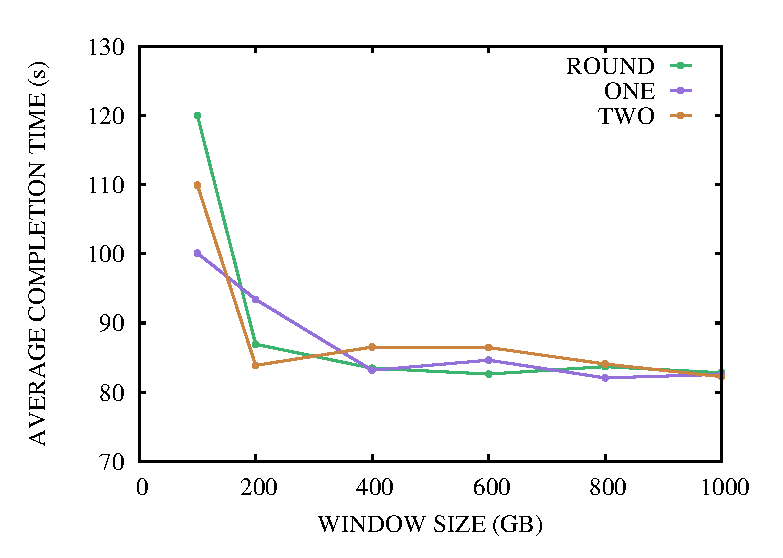
\includegraphics[scale=0.41]{figures/window_size_time.eps}
\caption{Impact of the observation window size.}
\label{fig:time_windowsize}
\end{figure} 